%%!TEX program = xelatex
%%========================================================================================================
%% Material CV
%% Author: Artur Gomes
%%
%% Description: This template design was based on the
%% Google Material Design for the new Android 5.0 L 
%% version.
%%
%% Aknowledgements
%% The font used was the font Roboto used in Android:
%% http://developer.android.com/design/style/typography.html
%% 
%% Used the elegant font iconset for icons (colors were changed acording to the color of the separator):
%% http://www.flaticon.com/packs/elegant-font
%%========================================================================================================
% http://tex.stackexchange.com/questions/140960/custom-shadow-border-effect-with-tikz

\documentclass{article}
\usepackage{tikz}
%\usepackage{fontspec}
\usepackage[sfdefault]{roboto}
\usepackage[top=0cm, bottom=2cm, outer=0cm, inner=0cm]{geometry}
\usepackage[pages=some]{background}
\usepackage{materialCard}
\usepackage{multicol}
\usepackage{url}
\usepackage[utf8]{inputenc}
\usepackage{pagecolor,lipsum}% http://ctan.org/pkg/{pagecolor,lipsum}
\usepackage[T1]{fontenc}

\backgroundsetup{scale=1, color=black, opacity=1, placement=top, angle=0, contents={%
  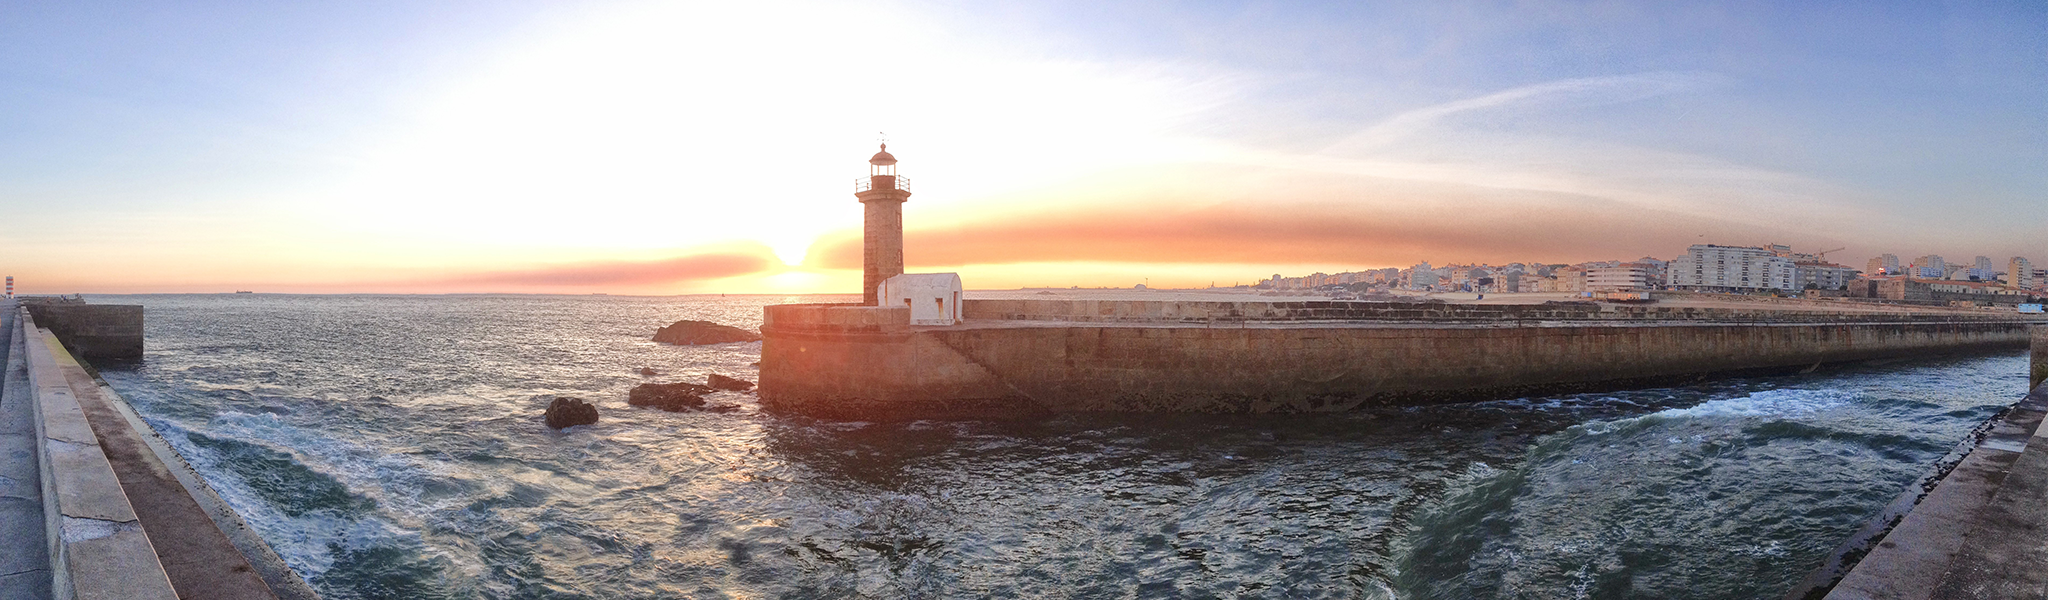
\includegraphics[width=\paperwidth,height=250pt]{images/pic}
  }}
\begin{document}
\pagecolor{MaterialGrey200}

\begin{minipage}[t]{\paperwidth}
	\pagenumbering{gobble}
	\Large
	\BgThispage
\end{minipage}
%\LARGE
%\noindent\colorbox{MaterialGreen}
%{\parbox[c][25pt][c]{\textwidth}{\hspace{15pt}\textcolor{white}{Contacts}}} %%Contacts separator
\hspace*{10pt} 
\begin{minipage}[t]{\paperwidth}
	\large

	\vspace*{20pt} 
	\begin{multicols}{2}
	%\materialCard[topimage=images/profile2,topcolor=MaterialRed500, cardwidth=0.25\paperwidth, topheight=76pt]{%!TEX root = cv.tex

\large
\begin{minipage}[t]{0.2\paperwidth}
\textcolor{MaterialBlue500}{
First Name Last Name
\vspace{5pt}
}\end{minipage}}
	%!TEX root = cv.tex

\large
\begin{minipage}[t]{0.2\paperwidth}
\textcolor{MaterialBlue500}{
First Name Last Name
\vspace{5pt}
}\end{minipage}
	\columnbreak
	%!TEX root = pic.tex

\newcommand{\ContactEntry}[2]{
	$\begin{array}{l}
	{\includegraphics[height=15pt]{#1}}
	\end{array}
	$ #2
}


\LARGE
\noindent\colorbox{materialGreen}
{\parbox[c][25pt][c]{\textwidth}{\hspace{15pt}\textcolor{white}{Contacts}}} %%Contacts separator

\begin{multicols}{2}

%%Contact Information
\large
%Add new or alter contact entries in this section by using the examples below
%for other contact information search the image folder for other icons
\ContactEntry{images/green/telephone1}{111-222-3333}

\ContactEntry{images/green/mail9}{mail@mail.com}

\ContactEntry{images/green/links1}{http://mywebsite.com}

\ContactEntry{images/green/linkedin2}{https://www.linkedin.com/in/amngomes}

\columnbreak

\ContactEntry{images/green/house3}{Street, number

\hspace*{25pt} City, State 0000-0000

\hspace*{25pt} Country}


\end{multicols}

	\end{multicols}{}
	\vspace{3pt}
	\large
	\materialCard[title=Experience, topcolor=MaterialRed500]{%!TEX root = material_cv.tex

%%Command used in order to make each entry cleaner
\normalsize
\newcommand{\ExperienceEntry}[5]{
\begin{tabular}{  p{\dimexpr 0.15\linewidth-2\tabcolsep} 
                   p{\dimexpr 0.75\linewidth-2\tabcolsep}}
  \textbf{\textcolor{MaterialRed900}{#1-}}\textbf{\textcolor{MaterialRed700}{#2}} & \textbf{#3}\\
  	& \normalsize #4\\
  	&{\small \textcolor{MaterialGrey500}{#5}}
  	\vspace*{2pt}
\end{tabular}
}

%\LARGE
%\noindent\colorbox{materialRed}
%{\parbox[c][25pt][c]{\textwidth}{\hspace{15pt}\textcolor{white}{Experience}}} %%Contacts separator
\begin{minipage}[t]{0.85\linewidth}
%%Contact Information
\normalsize
%Add new or alter education entries in this section by using the examples below
%\ExperienceEntry{starting year}{final year}{Position}{position description if applicable}{Place}
\ExperienceEntry{2007}{2016}{Position 0}{Job description....}{Place x}
\ExperienceEntry{2016}{2017}{Position 1}{Job description....}{Place y}
\end{minipage}
}{}

	\large
	\vspace{5pt}
	\materialCard[title=Education, topcolor=MaterialBlue500]{%!TEX root = cv.tex

%%Command used in order to make each entry cleaner
\newcommand{\EducationEntry}[5]{
\begin{tabular}{  p{\dimexpr 0.15\linewidth-2\tabcolsep} 
                   p{\dimexpr 0.70\linewidth-2\tabcolsep}}
  \textbf{\textcolor{materialBlueDark}{#1-}}\textbf{\textcolor{materialBlue}{#2}}\hspace{20pt} & \textbf{#3}\\
  	& \normalsize #4\\
  	&{\small \textcolor{textLightGray}{#5}}
\end{tabular}
\vspace*{10pt}
}

\LARGE
\noindent\colorbox{materialBlue}
{\parbox[c][25pt][c]{\textwidth}{\hspace{15pt}\textcolor{white}{Education}}} %%Contacts separator

%%Contact Information
\large
\vspace*{10pt}
%Add new or alter education entries in this section by using the examples below
%\EducationEntry{starting year}{final year}{Type of studies}{Studies description if applicable}{Place of studies}
\EducationEntry{2000}{2014}{Studies in something 1}{Studies description....}{Place X}

\vspace*{5pt}}


	\large
	\vspace{5pt}
	\materialCard[title=Competences, topcolor=MaterialAmber500]{%!TEX root = material_cv.tex
\normalsize
\newcommand{\InterestEntry}[4]{
\begin{tabular}{p{\dimexpr 0.3\linewidth-2\tabcolsep} 
                p{\dimexpr #4\linewidth-2\tabcolsep}}
  \textbf{\textcolor{MaterialOrange900}{#1}}\textbf{\textcolor{MaterialOrange700}{#2}} &\normalsize #3\\
\end{tabular}
}


%\Large
%\noindent\colorbox{materialBlue}
%{\parbox[c][25pt][c]{\textwidth}{\textcolor{white}{\textbf{Competences}}}} %%Contacts separator
\begin{minipage}[t]{0.85\linewidth}
\large
%\textcolor{MaterialAmber700}{\textbf{Program\textcolor{MaterialGrey700}{ming}}}
\normalsize

%%Contact Information
\InterestEntry{professional}{interests}{list of professional interests....}{0.85}
\InterestEntry{personal}{interests}{list of personal interests....}{0.85}

\end{minipage}



%%Contact Information
%\large
%\vspace*{10pt}
%
%\textcolor{materialBlue}{\textbf{Profes}}\textcolor{textGray}{\textbf{sional:}}\\
%\textBox{
%professional interests.... %%edit professional interest here
%}\\
%
%\textcolor{materialBlue}{\textbf{Pers}}\textcolor{textGray}{\textbf{onal:}}\\
%\textBox{
%personal interests....%%edit professional interest here
%}\\
%
%\vspace*{10pt}}

	\large
	\vspace{5pt}
	\materialCard[title=Awards, topcolor=MaterialPurple500]{%!TEX root = cv.tex

%%Command used in order to make each entry cleaner
\normalsize
\newcommand{\AwardEntry}[4]{
\begin{tabular}{p{\dimexpr 0.15\linewidth-2\tabcolsep} 
                p{\dimexpr 0.50\linewidth-2\tabcolsep}
                p{\dimexpr 0.25\linewidth-2\tabcolsep}}
  \textbf{\textcolor{MaterialPurple500}{#1}}\hspace{20pt} & \textbf{#2} & {\small \textcolor{MaterialGrey500}{#4}}\\
  	& \normalsize #3\\
\end{tabular}
}

%\LARGE
%\noindent\colorbox{MaterialPurple500}
%{\parbox[c][25pt][c]{\textwidth}{\hspace{15pt}\textcolor{white}{Awards}}} %%Contacts separator

%%Contact Information
\large
\begin{minipage}[t]{0.85\linewidth}
%Add new or alter education entries in this section by using the examples below
%\EducationEntry{starting year}{final year}{Type of studies}{Studies description if applicable}{Place of studies}
\AwardEntry{2000}{Studies in something 1}{Studies description....}{Place X}
\AwardEntry{2000}{Studies in something 1}{Studies description....}{Place X}
\end{minipage}}

%	\large
%	\vspace{5pt}
%	\materialCard[title=Awards, topcolor=MaterialPurple500]{%!TEX root = cv.tex

%%Command used in order to make each entry cleaner
\normalsize
\newcommand{\AwardEntry}[4]{
\begin{tabular}{p{\dimexpr 0.15\linewidth-2\tabcolsep} 
                p{\dimexpr 0.50\linewidth-2\tabcolsep}
                p{\dimexpr 0.25\linewidth-2\tabcolsep}}
  \textbf{\textcolor{MaterialPurple500}{#1}}\hspace{20pt} & \textbf{#2} & {\small \textcolor{MaterialGrey500}{#4}}\\
  	& \normalsize #3\\
\end{tabular}
}

%\LARGE
%\noindent\colorbox{MaterialPurple500}
%{\parbox[c][25pt][c]{\textwidth}{\hspace{15pt}\textcolor{white}{Awards}}} %%Contacts separator

%%Contact Information
\large
\begin{minipage}[t]{0.85\linewidth}
%Add new or alter education entries in this section by using the examples below
%\EducationEntry{starting year}{final year}{Type of studies}{Studies description if applicable}{Place of studies}
\AwardEntry{2000}{Studies in something 1}{Studies description....}{Place X}
\AwardEntry{2000}{Studies in something 1}{Studies description....}{Place X}
\end{minipage}}
\end{minipage}
%\materialCard[title=Mater222222222222222222222222222ial123Card, image=MaterialRed500]{\begin{tabular}{c} This node \\ is \\ valuable \end{tabular}}{card2}\\\\
\end{document}